\documentclass[a4paper,12pt]{article}
\usepackage{amsmath}
\usepackage{enumitem}
\usepackage{geometry}
\usepackage{esvect}
\usepackage{textcomp}
\usepackage{siunitx}
\usepackage{microtype}
\usepackage{parskip}
\usepackage{graphicx}

\begin{document}
   \null\hfill\begin{tabular}[t]{l@{}}
      \textbf{Nama: Aldzikri Dwijayanto P.} \\
      \textbf{NIM:\@ 195410189} \\
      \textbf{Kelas: TI-4}
   \end{tabular} 

   Dengan $\varepsilon_{s}=0,1\%$ lanjutkan komputasi pada contoh, sehingga dipenuhi $\varepsilon_{a}<\varepsilon_{s}$
   atau sampai iterasi ke-5\\
   \begin{itemize}
     \item Iterasi 1
        \begin{flalign*}
           x_{l}=2,8&\to f(x_{l})=-0,9(2,8)^{2}+1,7(2,8)+2,5\\
           x_{u}=3&\to f(x_{u})=-0,9(3)^{2}+1,7(3)+2,5\\
        \end{flalign*}

         \begin{flalign*}
            x_{r}=\frac{x_{l}+x_{u}}{2}=\frac{2,8+3}{2}=2,9\\
         \end{flalign*}

         \begin{flalign*}
            f(x_{r})&=-0,9(2,9)^{2}+1,7(2,9)+2,5\\
            &=-0,139
         \end{flalign*}

         \begin{flalign*}
            f(x_{r})&=-0,9(2,9)^{2}+1,7(2,9)+2,5\\
            &=-0,139\\
            f(x_{l}) \times f(x_{r})&=0,204\times (-0,139)\\
            &=0,028356<0\to\intertext{kondisi a langkah 3}
         \end{flalign*}

     \item Iterasi 2
        \begin{flalign*}
           x_{l}&=2,8\\
           x_{u}&=2,9\\
        \end{flalign*}

         \begin{flalign*}
            x_{r^{2}}&=\frac{x_{l}+x_{u}}{2}\\ 
            &=\frac{2,8+2,9}{2}\\
            &=2,85\\
         \end{flalign*}

         \begin{flalign*}
            f(x_{r^{2}})&=-0,9(2,85)^{2}+1,7(2,85)+2,5=0,03475\\
            f(x_{l})\times f(x_{r^{2}})&=0,204\times 0,03475=0,007089>0\to\intertext{kondisi
            $x_{l}=x_{r}$}
         \end{flalign*}

      \item Iterasi 3
         \begin{flalign*}
            x_{l}&=2,85\\
            x_{u}&=2,9
         \end{flalign*}

         \begin{flalign*}
            x_{r^{3}}&=\frac{x_{l}+x_{u}}{2}\\
            &=\frac{2,85+2,9}{2}\\
            &=2,875
         \end{flalign*}

         \begin{flalign*}
            f(x_{r^{3}})&=-0,9(2,875)^{2}+1,7(2,875)+2,5=-0,0515625\\ 
            f(x_{l})\times f(x_{r^{3}})&=0,007089 \times (-0,0515625)\\
            &=-0,0003655<0 \intertext{kondisi $x_{u}=x_{r}$}
         \end{flalign*}

      \item Iterasi 4
         \begin{flalign*}
            x_{l}&=2,85\\
            x_{u}&=2,875
         \end{flalign*}

         \begin{flalign*}
            x_{r^{4}}=\frac{x_{l}+x_{u}}{2}\\
            &=\frac{2,85+2,875}{2}\\
            &=2,8625
         \end{flalign*}

         \begin{flalign*}
            f(x_{r^{4}})&=-0,9(2,8625)+1,7(2,8625)+2,5\\
            &=-0,008265625\\
            f(x_{l})\times f(x_{r^{4}})&=0,007089 \times (-0,008265625)\\
            &=-0,000058595<0 \intertext{kondisi$x_{u}=x_{r}$}
         \end{flalign*}

         \item Iterasi 5
         \begin{flalign*}
            x_{l}&=2,85\\
            x_{u}&=2,8625
         \end{flalign*}

         \begin{flalign*}
            x_{r^{5}}=\frac{x_{l}+x_{u}}{2}\\
            &=\frac{2,85+2,8625}{2}\\
            &=2,85625
         \end{flalign*}

         \begin{flalign*}
            f(x_{r^{5}})&=-0,9(2,8625)^{2}+1,7(2,8625)+2,5\\
            &=-0,013277\\
            f(x_{l})\times f(x_{r^{5}})&=0,007089 \times 0,013277\\
            &=-0,0009412 \intertext{kondisi$x_{l}=x_{r}$}
         \end{flalign*}

         \item Iterasi 6
         \begin{flalign*}
            x_{l}&=2,85625\\
            x_{u}&=2,8625
         \end{flalign*}

         \begin{flalign*}
            x_{r^{6}}=\frac{x_{l}+x_{u}}{2}\\
            &=\frac{2,85625+2,8625}{2}\\
            &=2,859375
         \end{flalign*}

         \begin{flalign*}
            f(x_{r^{6}})&=-0,9(2,859375)+1,7(2,859375)+2,5\\
            &=-0,0251465\\
            f(x_{l})\times f(x_{r^{6}})&=0,0009412 \times 0,00251465\\
            &=-0,0000023668 \intertext{kondisi$x_{l}=x_{r}$}
         \end{flalign*}

         \item Iterasi 7
         \begin{flalign*}
            x_{l}&=2,859375\\
            x_{u}&=2,8625
         \end{flalign*}

         \begin{flalign*}
            x_{r^{7}}=\frac{x_{l}+x_{u}}{2}\\
            &=\frac{2,859375+2,8625}{2}\\
            &=2,8609375
         \end{flalign*}

         \begin{flalign*}
            f(x_{r^{7}})&=-0,9(2,8609375)^{2}+1,7(2,8609375)+2,5\\
            &=-0,00287329\\
            f(x_{l})\times f(x_{r^{7}})&=0,00251465 \times (-0,00251465)\\
            &=-0,000007225 \intertext{kondisi$x_{u}=x_{r}$}
         \end{flalign*}
   \end{itemize}

   \begin{flalign*}
      \varepsilon_{a}&=\left| \frac{x_{r^{7}}-x_{r^{6}}}{x_{r^{7}}} \right| \times 100\%\\
      &=\left| \frac{2,8609375 \times 2,859375}{2,8609375} \right| \times 100\%\\
   \end{flalign*}

   \newpage
   Flowchart program persamaan kuadrat
   \begin{center}
      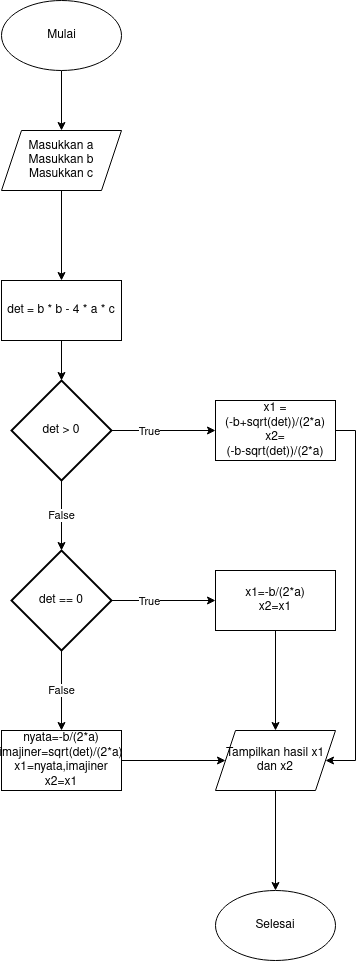
\includegraphics[scale=.5]{Numerik04.png}
   \end{center}
\newpage
   Program
   \begin{center}
      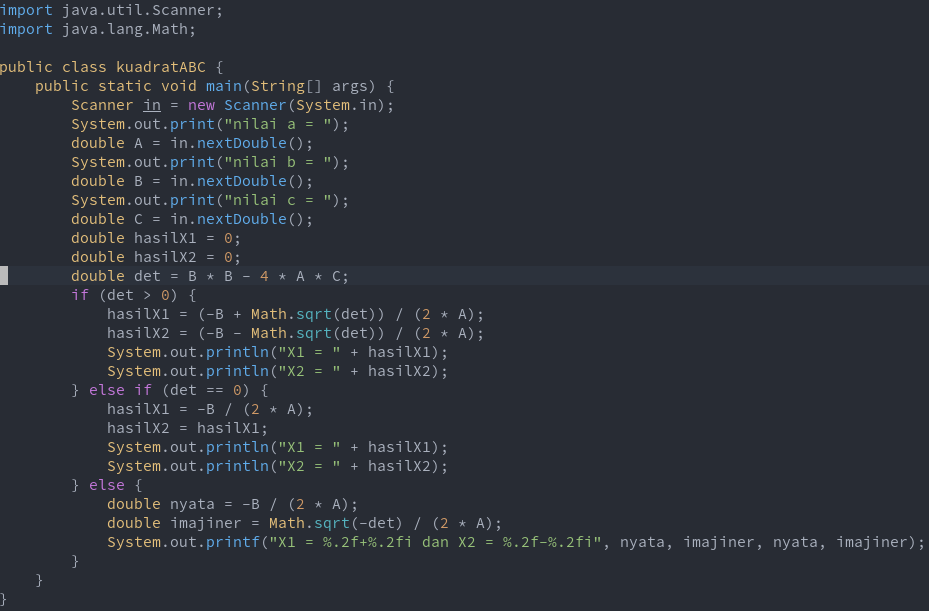
\includegraphics[scale=.5]{num04a.png} 
      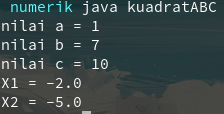
\includegraphics[scale=.7]{num04b.png} 
   \end{center}

   \newpage
   Algoritma metode bisection
   \begin{enumerate}
      \item Definisikan fungsi f(x) yang akan dicari akarnya.
         \item Tentukan nilai a dan b
            \item Tentukan torelansi e dan iterasi maksimum N
               \item Tentukan torelansi e dan iterasi maksimum N
               \item Jika f(a).f(b)>0 maka proses dihentikan karena tidak ada akar, bila tidak dilanjutkan.
                  \item Hitung f(x)
                     \item Bila f(x).f(a)<0 maka b=x dan f(b)=f(x), bila tidak a=x dan f(a)=f(x)
                     \item Jika |b-a|<e atau iterasi>iterasi maksimum maka proses dihentikan dan didapatkan akar = x, dan bila tidak, ulangi langkah 6.
   \end{enumerate}

  
\end{document}
